\documentclass{article}
\oddsidemargin -0.2cm
\evensidemargin -1.2cm
\textwidth 17cm
\headheight 2.2cm
\topmargin -4cm
\textheight 23cm
\usepackage[utf8]{inputenc}
\usepackage{amsmath}
\usepackage{amssymb}
\usepackage{multicol}
\usepackage{hyperref}
\usepackage{enumitem}
\usepackage{blindtext}
\usepackage{graphicx}
\graphicspath{ {figures/} }

\begin{document}

\author{Anthony Liu}
\title{Predicting solar installation rates using demographic data}
\maketitle

\section{Introduction / Business Problem}

The central problem that the analysis in this report will attempt to address is "Can we predict solar installation rates in the different local government areas of Australia using demographic data?". As the effects of global climate change are becoming better understood, the move towards renewable energy sources has become an important focus \cite{ipcc}. Solar energy is emerging as one of the most popular forms of renewable energy for reasons such as decreasing costs, environmental ethics, health, government incentives and accessibility \cite{pew, seia}. \\

Australia is in a particularly privileged position to have some of the best solar energy resources in the world \cite{geogov}. Being able to answer the proposed question may lead to insights which guide policy, investment or further research to better utilise this natural resource. Given that installation of solar constitutes a purchase and purchases are made by individuals under their own unique circumstances, there is good reason to believe that demographic factors (such as financial status, dwelling structure, education, etc.) may affect installation rates. In this analysis we limit our scope to prediction of solar installation rates in each local government area (LGA) based on available demographic data. Questions of inference such as which specific demographic factors are related to installation rates are not considered. \\

Parties who may be interested in this problem include policy makers, investors and researchers. Reliable predictions on installation rates may guide projections and highlight both the level and content of policy intervention justified in affecting solar uptake. Also, investors in the solar industry hold an advantage if they have reliable guidance on which local government areas in the future (accounting for demographic shifts) are likely to install solar. Finally, results from attempting to answer this question may lead to new lines of inquiry among researchers (e.g. if we can indeed predict installation rates then that provides justification to then do further research on which exact demographic factors have an effect).

\section{Data}

To answer our problem we will consider two separate types of data: data regarding solar installation rates in each LGA and data regarding demographics in each LGA. We obtain our first dataset on solar installations from the Australian Photovoltaic Institute \cite{pvdata}. The Australian Photovoltatic Institute (APVI) is a not-for-profit company whose stated objective is to "Support the increased development and use of PV via research, analysis and information" \cite{apvi}. The photovoltaic (PV) data by the APVI was compiled from Australian government body sources: PV installation data came from the Clean Energy Regulator \cite{pvdata, ceg} and attached LGA data was from the Australian Bureau of Statistics (ABS) \cite{pvdata, abspv}. Of particular interest to this analysis is the density variable, an estimate of the percentage of dwellings in each LGA which have installed solar systems. \\

Detailed demographic data on each LGA including socio-economic indicators, dwelling structure, age, sex, cultural background, education and employment was also obtained from the ABS \cite{abs}. In addition, we also attempt to include geographical features of each LGA using data from the Foursquare API. Figures \ref{fig:fig1} and \ref{fig:fig2} provide a preview of how the socio-economic indicators and education/employment data look on the ABS website respectively. These entries will later be wrangled into an appropriate format and act as individual features/predictors of a machine learning algorithm to predict density (i.e. solar installation rate in each LGA).

\begin{figure}
  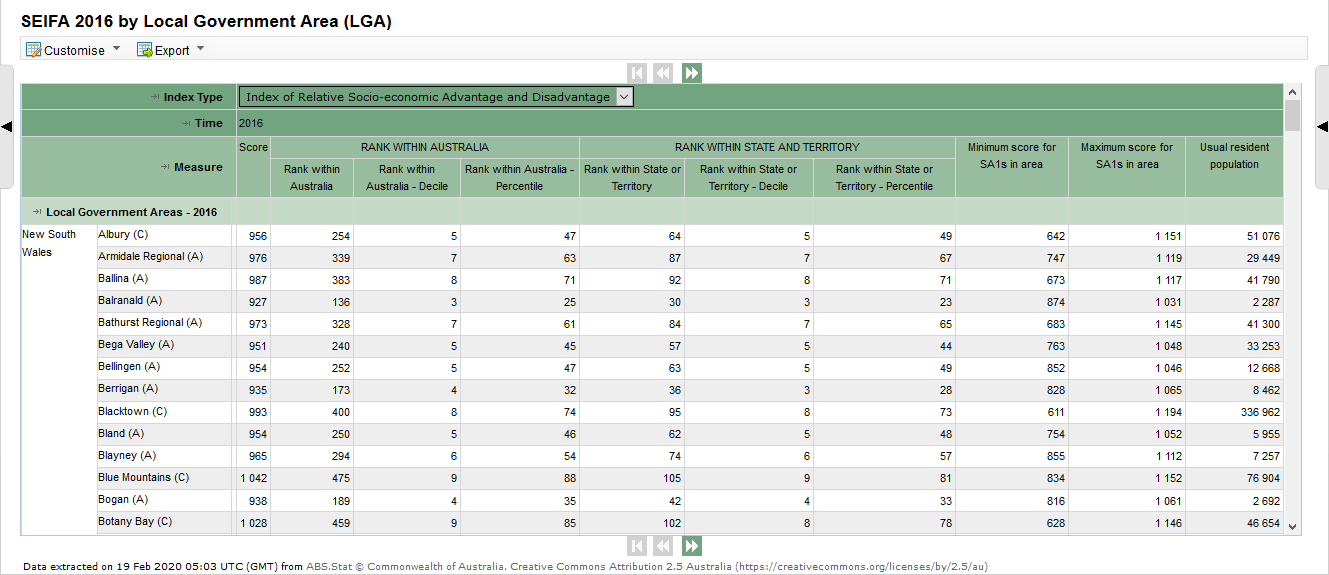
\includegraphics[width=\linewidth]{fig1.png}
  \caption{A preview of the socio-economic indicators dataset on the ABS website, prior to exporting as a CSV file and performing data wrangling}
  \label{fig:fig1}
\end{figure}

\begin{figure}
  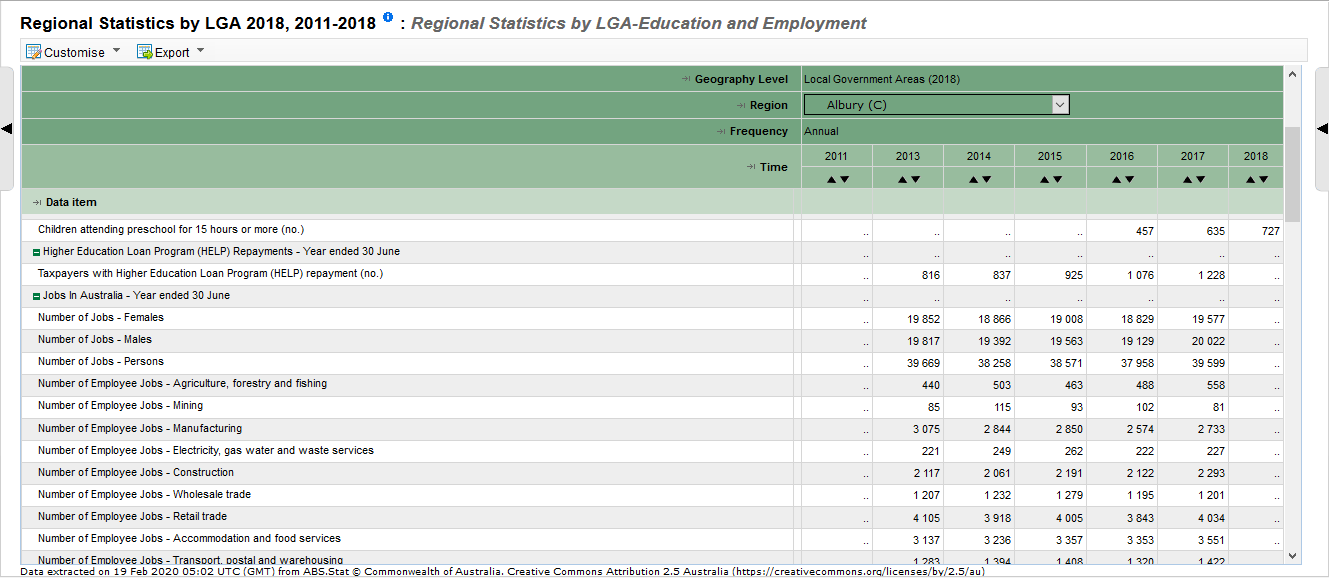
\includegraphics[width=\linewidth]{fig2.png}
  \caption{A preview of the education and employment dataset on the ABS website, prior to exporting as a CSV file and performing data wrangling}
  \label{fig:fig2}
\end{figure}

\medskip

\begin{thebibliography}{9}

\bibitem{ipcc} 
\url{https://www.ipcc.ch/report/renewable-energy-sources-and-climate-change-mitigation/}

\bibitem{pew} 
\url{https://www.pewresearch.org/fact-tank/2016/10/05/americans-strongly-favor-expanding-solar-power-to-help-address-costs-and-environmental-concerns/}

\bibitem{seia}
\url{https://www.seia.org/solar-industry-research-data}

\bibitem{geogov} 
\url{https://www.ga.gov.au/scientific-topics/energy/resources/other-renewable-energy-resources/solar-energy}

\bibitem{pvdata}
Australian PV Institute (APVI) Solar Map, funded by the Australian Renewable Energy Agency, accessed from pv-map.apvi.org.au on 19 February 2020. Dataset can be downloaded from \url{https://pv-map.apvi.org.au/historical#4/-26.67/134.12}

\bibitem{apvi}
\url{http://apvi.org.au/about-us/}

\bibitem{ceg}
\url{http://www.cleanenergyregulator.gov.au/RET/Forms-and-resources/Postcode-data-for-small-scale-installations}

\bibitem{abspv}
\url{https://www.abs.gov.au/AUSSTATS/abs@.nsf/DetailsPage/1270.0.55.003July%202016?OpenDocument}

\bibitem{abs}
\url{http://stat.data.abs.gov.au/}

\end{thebibliography}

\end{document}